%
% 6.006 problem set 2
%
\documentclass[12pt,twoside]{article}

% Cross-references for handout numbers.

% Updated to include SMA course for Fall 2001 -- cel

\newcommand{\name}{}


\usepackage{latexsym}
%\usepackage{bbm}
\usepackage{times,url}
\usepackage{clrscode3e}

\newcommand{\mitst}[1]{\begin{description}
\item[MIT students:] #1
\end{description}}
\newcommand{\smast}[1]{\begin{description}
\item[SMA students:] #1
\end{description}}

\newcommand{\profs}{Professors Erik Demaine and Srini Devadas}
\newcommand{\subj}{6.006}

\newlength{\toppush}
\setlength{\toppush}{2\headheight}
\addtolength{\toppush}{\headsep}

\newcommand{\htitle}[2]{\noindent\vspace*{-\toppush}\newline\parbox{6.5in}
{\textit{Introduction to Algorithms: 6.006}\hfill\name\newline
Massachusetts Institute of Technology \hfill #2\newline
\profs\hfill #1 \vspace*{-.5ex}\newline
\mbox{}\hrulefill\mbox{}}\vspace*{1ex}\mbox{}\newline
\begin{center}{\Large\bf #1}\end{center}}

\newcommand{\handout}[2]{\thispagestyle{empty}
 \markboth{#1}{#1}
 \pagestyle{myheadings}\htitle{#1}{#2}}

\newcommand{\htitlewithouttitle}[2]{\noindent\vspace*{-\toppush}\newline\parbox{6.5in}
{\textit{Introduction to Algorithms}\hfill#2\newline
Massachusetts Institute of Technology \hfill 6.006\newline
%Singapore-MIT Alliance \hfill SMA5503\newline
\profs\hfill Handout #1\vspace*{-.5ex}\newline
\mbox{}\hrulefill\mbox{}}\vspace*{1ex}\mbox{}\newline}

\newcommand{\handoutwithouttitle}[2]{\thispagestyle{empty}
 \markboth{Handout \protect\ref{#1}}{Handout \protect\ref{#1}}
 \pagestyle{myheadings}\htitlewithouttitle{\protect\ref{#1}}{#2}}

\newcommand{\exam}[2]{% parameters: exam name, date
 \thispagestyle{empty}
 \markboth{\subj\ #1\hspace{1in}Name\hrulefill\ \ }%
          {\subj\ #1\hspace{1in}Name\hrulefill\ \ }
 \pagestyle{myheadings}\examtitle{#1}{#2}
 \renewcommand{\theproblem}{Problem \arabic{problemnum}}
}
\newcommand{\examsolutions}[3]{% parameters: handout, exam name, date
 \thispagestyle{empty}
 \markboth{Handout \protect\ref{#1}: #2}{Handout \protect\ref{#1}: #2}
% \pagestyle{myheadings}\htitle{\protect\ref{#1}}{#2}{#3}
 \pagestyle{myheadings}\examsolutionstitle{\protect\ref{#1}} {#2}{#3}
 \renewcommand{\theproblem}{Problem \arabic{problemnum}}
}
\newcommand{\examsolutionstitle}[3]{\noindent\vspace*{-\toppush}\newline\parbox{6.5in}
{\textit{Introduction to Algorithms}\hfill#3\newline
Massachusetts Institute of Technology \hfill 6.006\newline
%Singapore-MIT Alliance \hfill SMA5503\newline
\profs\hfill Handout #1\vspace*{-.5ex}\newline
\mbox{}\hrulefill\mbox{}}\vspace*{1ex}\mbox{}\newline
\begin{center}{\Large\bf #2}\end{center}}

\newcommand{\takehomeexam}[2]{% parameters: exam name, date
 \thispagestyle{empty}
 \markboth{\subj\ #1\hfill}{\subj\ #1\hfill}
 \pagestyle{myheadings}\examtitle{#1}{#2}
 \renewcommand{\theproblem}{Problem \arabic{problemnum}}
}

\makeatletter
\newcommand{\exambooklet}[2]{% parameters: exam name, date
 \thispagestyle{empty}
 \markboth{\subj\ #1}{\subj\ #1}
 \pagestyle{myheadings}\examtitle{#1}{#2}
 \renewcommand{\theproblem}{Problem \arabic{problemnum}}
 \renewcommand{\problem}{\newpage
 \item \let\@currentlabel=\theproblem
 \markboth{\subj\ #1, \theproblem}{\subj\ #1, \theproblem}}
}
\makeatother


\newcommand{\examtitle}[2]{\noindent\vspace*{-\toppush}\newline\parbox{6.5in}
{\textit{Introduction to Algorithms}\hfill#2\newline
Massachusetts Institute of Technology \hfill 6.006 Fall 2009\newline
%Singapore-MIT Alliance \hfill SMA5503\newline
\profs\hfill #1\vspace*{-.5ex}\newline
\mbox{}\hrulefill\mbox{}}\vspace*{1ex}\mbox{}\newline
\begin{center}{\Large\bf #1}\end{center}}

\newcommand{\grader}[1]{\hspace{1cm}\textsf{\textbf{#1}}\hspace{1cm}}

%\newcommand{\points}[1]{[#1 points]\ }
\newcount\pointcount
\newcommand{\points}[1]{\pointcount=#1\relax \ifnum\pointcount=1 [#1 point]\else [#1 points]\fi\ }

\newcommand{\parts}[1]
{
  \ifnum#1=1
  (1 part)
  \else
  (#1 parts)
  \fi
  \ 
}

\newcommand{\bparts}{\begin{problemparts}}
\newcommand{\eparts}{\end{problemparts}}
\newcommand{\ppart}{\problempart}

%\newcommand{\lg} {lg\ }

\setlength{\oddsidemargin}{0pt}
\setlength{\evensidemargin}{0pt}
\setlength{\textwidth}{6.5in}
\setlength{\topmargin}{0in}
\setlength{\textheight}{8.5in}


\renewcommand{\cases}[1]{\left\{ \begin{array}{ll}#1\end{array}\right.}
\newcommand{\cif}[1]{\mbox{if $#1$}}
\newcommand{\cwhen}[1]{\mbox{when $#1$}}

\newcounter{problemnum}
\newcommand{\theproblem}{Problem \theproblemsetnum-\arabic{problemnum}}
\newenvironment{problems}{
        \begin{list}{{\bf \theproblem. \hspace*{0.5em}}}
        {\setlength{\leftmargin}{0em}
         \setlength{\rightmargin}{0em}
         \setlength{\labelwidth}{0em}
         \setlength{\labelsep}{0em}
         \usecounter{problemnum}}}{\end{list}}
\makeatletter
\newcommand{\problem}[1][{}]{\item \let\@currentlabel=\theproblem \textbf{#1}}
\makeatother

\newcounter{problempartnum}[problemnum]
\newenvironment{problemparts}{
        \begin{list}{{\bf (\alph{problempartnum})}}
        {\setlength{\leftmargin}{2.5em}
         \setlength{\rightmargin}{2.5em}
         \setlength{\labelsep}{0.5em}}}{\end{list}}
\newcommand{\problempart}{\addtocounter{problempartnum}{1}\item}

\newenvironment{truefalseproblemparts}{
        \begin{list}{{\bf (\alph{problempartnum})\ \ \ T\ \ F\hfil}}
        {\setlength{\leftmargin}{4.5em}
         \setlength{\rightmargin}{2.5em}
         \setlength{\labelsep}{0.5em}
         \setlength{\labelwidth}{4.5em}}}{\end{list}}

\newcounter{exercisenum}
\newcommand{\theexercise}{Exercise \theproblemsetnum-\arabic{exercisenum}}
\newenvironment{exercises}{
        \begin{list}{{\bf \theexercise. \hspace*{0.5em}}}
        {\setlength{\leftmargin}{0em}
         \setlength{\rightmargin}{0em}
         \setlength{\labelwidth}{0em}
         \setlength{\labelsep}{0em}
        \usecounter{exercisenum}}}{\end{list}}
\makeatletter
\newcommand{\exercise}{\item \let\@currentlabel=\theexercise}
\makeatother

\newcounter{exercisepartnum}[exercisenum]
%\newcommand{\problem}[1]{\medskip\mbox{}\newline\noindent{\bf Problem #1.}\hspace*{1em}}
%\newcommand{\exercise}[1]{\medskip\mbox{}\newline\noindent{\bf Exercise #1.}\hspace*{1em}}

\newenvironment{exerciseparts}{
        \begin{list}{{\bf (\alph{exercisepartnum})}}
        {\setlength{\leftmargin}{2.5em}
         \setlength{\rightmargin}{2.5em}
         \setlength{\labelsep}{0.5em}}}{\end{list}}
\newcommand{\exercisepart}{\addtocounter{exercisepartnum}{1}\item}


% Macros to make captions print with small type and 'Figure xx' in bold.
\makeatletter
\def\fnum@figure{{\bf Figure \thefigure}}
\def\fnum@table{{\bf Table \thetable}}
\let\@mycaption\caption
%\long\def\@mycaption#1[#2]#3{\addcontentsline{\csname
%  ext@#1\endcsname}{#1}{\protect\numberline{\csname 
%  the#1\endcsname}{\ignorespaces #2}}\par
%  \begingroup
%    \@parboxrestore
%    \small
%    \@makecaption{\csname fnum@#1\endcsname}{\ignorespaces #3}\par
%  \endgroup}
%\def\mycaption{\refstepcounter\@captype \@dblarg{\@mycaption\@captype}}
%\makeatother
\let\mycaption\caption
%\newcommand{\figcaption}[1]{\mycaption[]{#1}}

\newcounter{totalcaptions}
\newcounter{totalart}

\newcommand{\figcaption}[1]{\addtocounter{totalcaptions}{1}\caption[]{#1}}

% \psfigures determines what to do for figures:
%       0 means just leave vertical space
%       1 means put a vertical rule and the figure name
%       2 means insert the PostScript version of the figure
%       3 means put the figure name flush left or right
\newcommand{\psfigures}{0}
\newcommand{\spacefigures}{\renewcommand{\psfigures}{0}}
\newcommand{\rulefigures}{\renewcommand{\psfigures}{1}}
\newcommand{\macfigures}{\renewcommand{\psfigures}{2}}
\newcommand{\namefigures}{\renewcommand{\psfigures}{3}}

\newcommand{\figpart}[1]{{\bf (#1)}\nolinebreak[2]\relax}
\newcommand{\figparts}[2]{{\bf (#1)--(#2)}\nolinebreak[2]\relax}


\macfigures     % STATE

% When calling \figspace, make sure to leave a blank line afterward!!
% \widefigspace is for figures that are more than 28pc wide.
\newlength{\halffigspace} \newlength{\wholefigspace}
\newlength{\figruleheight} \newlength{\figgap}
\newcommand{\setfiglengths}{\ifnum\psfigures=1\setlength{\figruleheight}{\hruleheight}\setlength{\figgap}{1em}\else\setlength{\figruleheight}{0pt}\setlength{\figgap}{0em}\fi}
\newcommand{\figspace}[2]{\ifnum\psfigures=0\leavefigspace{#1}\else%
\setfiglengths%
\setlength{\wholefigspace}{#1}\setlength{\halffigspace}{.5\wholefigspace}%
\rule[-\halffigspace]{\figruleheight}{\wholefigspace}\hspace{\figgap}#2\fi}
\newlength{\widefigspacewidth}
% Make \widefigspace put the figure flush right on the text page.
\newcommand{\widefigspace}[2]{
\ifnum\psfigures=0\leavefigspace{#1}\else%
\setfiglengths%
\setlength{\widefigspacewidth}{28pc}%
\addtolength{\widefigspacewidth}{-\figruleheight}%
\setlength{\wholefigspace}{#1}\setlength{\halffigspace}{.5\wholefigspace}%
\makebox[\widefigspacewidth][r]{#2\hspace{\figgap}}\rule[-\halffigspace]{\figruleheight}{\wholefigspace}\fi}
\newcommand{\leavefigspace}[1]{\setlength{\wholefigspace}{#1}\setlength{\halffigspace}{.5\wholefigspace}\rule[-\halffigspace]{0em}{\wholefigspace}}

% Commands for including figures with macpsfig.
% To use these commands, documentstyle ``macpsfig'' must be specified.
\newlength{\macfigfill}
\makeatother
\newlength{\bbx}
\newlength{\bby}
\newcommand{\macfigure}[5]{\addtocounter{totalart}{1}
\ifnum\psfigures=2%
\setlength{\bbx}{#2}\addtolength{\bbx}{#4}%
\setlength{\bby}{#3}\addtolength{\bby}{#5}%
\begin{flushleft}
\ifdim#4>28pc\setlength{\macfigfill}{#4}\addtolength{\macfigfill}{-28pc}\hspace*{-\macfigfill}\fi%
\mbox{\psfig{figure=./#1.ps,%
bbllx=#2,bblly=#3,bburx=\bbx,bbury=\bby}}
\end{flushleft}%
\else\ifdim#4>28pc\widefigspace{#5}{#1}\else\figspace{#5}{#1}\fi\fi}
\makeatletter

\newlength{\savearraycolsep}
\newcommand{\narrowarray}[1]{\setlength{\savearraycolsep}{\arraycolsep}\setlength{\arraycolsep}{#1\arraycolsep}}
\newcommand{\normalarray}{\setlength{\arraycolsep}{\savearraycolsep}}

\newcommand{\hint}{{\em Hint:\ }}

% Macros from /th/u/clr/mac.tex

\newcommand{\set}[1]{\left\{ #1 \right\}}
\newcommand{\abs}[1]{\left| #1\right|}
\newcommand{\card}[1]{\left| #1\right|}
\newcommand{\floor}[1]{\left\lfloor #1 \right\rfloor}
\newcommand{\ceil}[1]{\left\lceil #1 \right\rceil}
\newcommand{\ang}[1]{\ifmmode{\left\langle #1 \right\rangle}
   \else{$\left\langle${#1}$\right\rangle$}\fi}
        % the \if allows use outside mathmode,
        % but will swallow following space there!
\newcommand{\paren}[1]{\left( #1 \right)}
\newcommand{\bracket}[1]{\left[ #1 \right]}
\newcommand{\prob}[1]{\Pr\left\{ #1 \right\}}
\newcommand{\Var}{\mathop{\rm Var}\nolimits}
\newcommand{\expect}[1]{{\rm E}\left[ #1 \right]}
\newcommand{\expectsq}[1]{{\rm E}^2\left[ #1 \right]}
\newcommand{\variance}[1]{{\rm Var}\left[ #1 \right]}
\renewcommand{\choose}[2]{{{#1}\atopwithdelims(){#2}}}
\def\pmod#1{\allowbreak\mkern12mu({\rm mod}\,\,#1)}
\newcommand{\matx}[2]{\left(\begin{array}{*{#1}{c}}#2\end{array}\right)}
\newcommand{\Adj}{\mathop{\rm Adj}\nolimits}

\newtheorem{theorem}{Theorem}
\newtheorem{lemma}[theorem]{Lemma}
\newtheorem{corollary}[theorem]{Corollary}
\newtheorem{xample}{Example}
\newtheorem{definition}{Definition}
\newenvironment{example}{\begin{xample}\rm}{\end{xample}}
\newcommand{\proof}{\noindent{\em Proof.}\hspace{1em}}
\def\squarebox#1{\hbox to #1{\hfill\vbox to #1{\vfill}}}
\newcommand{\qedbox}{\vbox{\hrule\hbox{\vrule\squarebox{.667em}\vrule}\hrule}}
\newcommand{\qed}{\nopagebreak\mbox{}\hfill\qedbox\smallskip}
\newcommand{\eqnref}[1]{(\protect\ref{#1})}

%%\newcommand{\twodots}{\mathinner{\ldotp\ldotp}}
\newcommand{\transpose}{^{\mbox{\scriptsize \sf T}}}
\newcommand{\amortized}[1]{\widehat{#1}}

\newcommand{\punt}[1]{}

%%% command for putting definitions into boldface
% New style for defined terms, as of 2/23/88, redefined by THC.
\newcommand{\defn}[1]{{\boldmath\textit{\textbf{#1}}}}
\newcommand{\defi}[1]{{\textit{\textbf{#1\/}}}}

\newcommand{\red}{\leq_{\rm P}}
\newcommand{\lang}[1]{%
\ifmmode\mathord{\mathcode`-="702D\rm#1\mathcode`\-="2200}\else{\rm#1}\fi}

%\newcommand{\ckt}[1]{\ifmmode\mathord{\mathcode`-="702D\sc #1\mathcode`\-="2200}\else$\mathord{\mathcode`-="702D\sc #1\mathcode`\-="2200}$\fi}
\newcommand{\ckt}[1]{\ifmmode \sc #1\else$\sc #1$\fi}

%% Margin notes - use \notesfalse to turn off notes.
\setlength{\marginparwidth}{0.6in}
\reversemarginpar
\newif\ifnotes
\notestrue
\newcommand{\longnote}[1]{
  \ifnotes
    {\medskip\noindent Note: \marginpar[\hfill$\Longrightarrow$]
      {$\Longleftarrow$}{#1}\medskip}
  \fi}
\newcommand{\note}[1]{
  \ifnotes
    {\marginpar{\tiny \raggedright{#1}}}
  \fi}


\newcommand{\reals}{\mathbbm{R}}
\newcommand{\integers}{\mathbbm{Z}}
\newcommand{\naturals}{\mathbbm{N}}
\newcommand{\rationals}{\mathbbm{Q}}
\newcommand{\complex}{\mathbbm{C}}

\newcommand{\oldreals}{{\bf R}}
\newcommand{\oldintegers}{{\bf Z}}
\newcommand{\oldnaturals}{{\bf N}}
\newcommand{\oldrationals}{{\bf Q}}
\newcommand{\oldcomplex}{{\bf C}}

\newcommand{\w}{\omega}                 %% for fft chapter

\newenvironment{closeitemize}{\begin{list}
{$\bullet$}
{\setlength{\itemsep}{-0.2\baselineskip}
\setlength{\topsep}{0.2\baselineskip}
\setlength{\parskip}{0pt}}}
{\end{list}}

% These are necessary within a {problems} environment in order to restore
% the default separation between bullets and items.
\newenvironment{normalitemize}{\setlength{\labelsep}{0.5em}\begin{itemize}}
                              {\end{itemize}}
\newenvironment{normalenumerate}{\setlength{\labelsep}{0.5em}\begin{enumerate}}
                                {\end{enumerate}}

%\def\eqref#1{Equation~(\ref{eq:#1})}
%\newcommand{\eqref}[1]{Equation (\ref{eq:#1})}
\newcommand{\eqreftwo}[2]{Equations (\ref{eq:#1}) and~(\ref{eq:#2})}
\newcommand{\ineqref}[1]{Inequality~(\ref{ineq:#1})}
\newcommand{\ineqreftwo}[2]{Inequalities (\ref{ineq:#1}) and~(\ref{ineq:#2})}

\newcommand{\figref}[1]{Figure~\ref{fig:#1}}
\newcommand{\figreftwo}[2]{Figures \ref{fig:#1} and~\ref{fig:#2}}

\newcommand{\liref}[1]{line~\ref{li:#1}}
\newcommand{\Liref}[1]{Line~\ref{li:#1}}
\newcommand{\lirefs}[2]{lines \ref{li:#1}--\ref{li:#2}}
\newcommand{\Lirefs}[2]{Lines \ref{li:#1}--\ref{li:#2}}
\newcommand{\lireftwo}[2]{lines \ref{li:#1} and~\ref{li:#2}}
\newcommand{\lirefthree}[3]{lines \ref{li:#1}, \ref{li:#2}, and~\ref{li:#3}}

\newcommand{\lemlabel}[1]{\label{lem:#1}}
\newcommand{\lemref}[1]{Lemma~\ref{lem:#1}} 

\newcommand{\exref}[1]{Exercise~\ref{ex:#1}}

\newcommand{\handref}[1]{Handout~\ref{#1}}

\newcommand{\defref}[1]{Definition~\ref{def:#1}}

% (1997.8.16: Victor Luchangco)
% Modified \hlabel to only get date and to use handouts counter for number.
%   New \handout and \handoutwithouttitle commands in newmac.tex use this.
%   The date is referenced by <label>-date.
%   (Retained old definition as \hlabelold.)
%   Defined \hforcelabel to use an argument instead of the handouts counter.

\newcounter{handouts}
\setcounter{handouts}{0}

\newcommand{\hlabel}[2]{%
\stepcounter{handouts}
{\edef\next{\write\@auxout{\string\newlabel{#1}{{\arabic{handouts}}{0}}}}\next}
\write\@auxout{\string\newlabel{#1-date}{{#2}{0}}}
}

\newcommand{\hforcelabel}[3]{%          Does not step handouts counter.
\write\@auxout{\string\newlabel{#1}{{#2}{0}}}
\write\@auxout{\string\newlabel{#1-date}{{#3}{0}}}}


% less ugly underscore
% --juang, 2008 oct 05
\renewcommand{\_}{\vrule height 0 pt depth 0.4 pt width 0.5 em \,}


\usepackage{amsmath}
\usepackage{url}
\usepackage{graphicx}
\usepackage{clrscode3e}

\newcommand{\answer}{
 \par\medskip
 \textbf{Answer:}
}

\newcommand{\collaborators}{ \textbf{Collaborators:}
%%% COLLABORATORS START %%%
None.
%%% COLLABORATORS END %%%
}

\newcommand{\answerIa}{ \answer
%%% PROBLEM 1(a) ANSWER START %%%
0
%%% PROBLEM 1(a) ANSWER END %%%
}

\newcommand{\answerIb}{ \answer
%%% PROBLEM 1(b) ANSWER START %%%
0
%%% PROBLEM 1(b) ANSWER END %%%
}

\newcommand{\answerIc}{ \answer
%%% PROBLEM 1(c) ANSWER START %%%
0
%%% PROBLEM 1(c) ANSWER END %%%
}

\newcommand{\answerId}{ \answer
%%% PROBLEM 1(d) ANSWER START %%%
0
%%% PROBLEM 1(d) ANSWER END %%%
}
\newcommand{\answerIe}{ \answer
%%% PROBLEM 1(e) ANSWER START %%%
0
%%% PROBLEM 1(e) ANSWER END %%%
}
\newcommand{\answerIf}{ \answer
%%% PROBLEM 1(f) ANSWER START %%%
0
%%% PROBLEM 1(f) ANSWER END %%%
}
\newcommand{\answerIg}{ \answer
%%% PROBLEM 1(g) ANSWER START %%%
0
%%% PROBLEM 1(g) ANSWER END %%%
}
\newcommand{\answerIh}{ \answer
%%% PROBLEM 1(h) ANSWER START %%%
0
%%% PROBLEM 1(h) ANSWER END %%%
}
\newcommand{\answerIi}{ \answer
%%% PROBLEM 1(i) ANSWER START %%%
0
%%% PROBLEM 1(i) ANSWER END %%%
}
\newcommand{\answerIj}{ \answer
%%% PROBLEM 1(j) ANSWER START %%%
0
%%% PROBLEM 1(j) ANSWER END %%%
}
\newcommand{\answerIk}{ \answer
%%% PROBLEM 1(k) ANSWER START %%%
0
%%% PROBLEM 1(k) ANSWER END %%%
}
\newcommand{\answerIl}{ \answer
%%% PROBLEM 1(l) ANSWER START %%%
0
%%% PROBLEM 1(l) ANSWER END %%%
}
\newcommand{\answerIm}{ \answer
%%% PROBLEM 1(m) ANSWER START %%%
0
%%% PROBLEM 1(m) ANSWER END %%%
}
\newcommand{\answerIn}{ \answer
%%% PROBLEM 1(n) ANSWER START %%%
0
%%% PROBLEM 1(n) ANSWER END %%%
}
\newcommand{\answerIo}{ \answer
%%% PROBLEM 1(o) ANSWER START %%%
0
%%% PROBLEM 1(o) ANSWER END %%%
}
\newcommand{\answerIp}{ \answer
%%% PROBLEM 1(p) ANSWER START %%%
0
%%% PROBLEM 1(p) ANSWER END %%%
}
\newcommand{\answerIq}{ \answer
%%% PROBLEM 1(q) ANSWER START %%%
0
%%% PROBLEM 1(q) ANSWER END %%%
}
\newcommand{\answerIr}{ \answer
%%% PROBLEM 1(r) ANSWER START %%%
0
%%% PROBLEM 1(r) ANSWER END %%%
}
\newcommand{\answerIs}{ \answer
%%% PROBLEM 1(s) ANSWER START %%%
0
%%% PROBLEM 1(s) ANSWER END %%%
}
\newcommand{\answerIt}{ \answer
%%% PROBLEM 1(t) ANSWER START %%%
0
%%% PROBLEM 1(t) ANSWER END %%%
}
\newcommand{\answerIu}{ \answer
%%% PROBLEM 1(u) ANSWER START %%%
Your proof in latex.
%%% PROBLEM 1(u) ANSWER END %%%
}
\newcommand{\answerIIa}{ \answer 
%%% PROBLEM 2(a) ANSWER START %%%
method\_name
%%% PROBLEM 2(a) ANSWER END %%%
}
\newcommand{\answerIIb}{ \answer
%%% PROBLEM 2(b) ANSWER START %%%
0
%%% PROBLEM 2(b) ANSWER END %%%
}
\newcommand{\answerIIc}{ \answer
%%% PROBLEM 2(c) ANSWER START %%%
0
%%% PROBLEM 2(c) ANSWER END %%%
}
\newcommand{\answerIId}{ \answer
%%% PROBLEM 2(d) ANSWER START %%%
0
%%% PROBLEM 2(d) ANSWER END %%%
}

\setlength{\oddsidemargin}{0pt}
\setlength{\evensidemargin}{0pt}
\setlength{\textwidth}{6.5in}
\setlength{\topmargin}{0in}
\setlength{\textheight}{8.5in}

\newcommand{\theproblemsetnum}{2}
\newcommand{\releasedate}{September 15, 2011}
\newcommand{\partaduedate}{Tuesday, September 27}
\newcommand{\tabUnit}{3ex}
\newcommand{\tabT}{\hspace*{\tabUnit}}

\begin{document}

\handout{Problem Set \theproblemsetnum}{\releasedate}

\textbf{Both theory and programming questions} are due {\bf \partaduedate} at
{\bf 11:59PM}.
%
Please submit your solutions on \texttt{http://alg.csail.mit.edu}. The site
will prompt you for your answers to the questions, so you do not need to create
a solution template. The site will be open for PS2 submissions by Thursday,
September 22. You don't need to wait until then to work on your solutions, and
we encourage you to start early.

Remember, your goal is to communicate. Full credit will be given only
to a correct solution which is described clearly. Convoluted and
obtuse descriptions might receive low marks, even when they are
correct. Also, aim for concise solutions, as it will save you time
spent on write-ups, and also help you conceptualize the key idea of
the problem.

We will provide the solutions to the problem set 10 hours after the problem set
is due, which you will use to find any errors in the proof that you submitted.
You will need to submit a critique of your solutions by \textbf{Thursday,
September 29th, 11:59PM}. Your grade will be based on both your solutions and
your critique of the solutions.

\medskip

\hrulefill

\collaborators

\begin{problems}

\problem \points{40} \textbf{Fractal Rendering}

You landed a consulting gig with Gopple, who is about to introduce a new line
of mobile phones with Retina HD displays, which are based on unicorn e-ink and thus
have infinite resolution. The high-level executives heard that fractals have
infinite levels of detail, and decreed that the new phones' background will be
the  \defn{Koch snowflake} (Figure \ref{fig:snowflake}).

\begin{figure}[htbp]
\centering
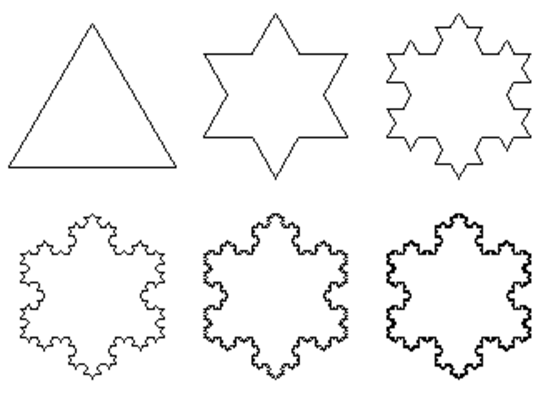
\includegraphics[width=0.4\textwidth]{figures/snowflake.pdf}
\caption{The Koch snowflake fractal, rendered at Level of Detail (LoD) 0 through 5.}
\label{fig:snowflake}
\end{figure}

Unfortunately, the phone's processor (CPU) and the graphics chip (GPU) powering
the display do not have infinite processing power, so the Koch fractal cannot be
rendered in infinite detail. Gopple engineers will stop the recursion at a
fixed depth $n$ in order to cap the processing requirement. 
For example, at $n=0$, the fractal is just a triangle.
Because higher depths result in more detailed drawing, this depth is usually
called the \defn{Level of Detail (LoD)}.

The Koch snowflake at LoD $n$ can be drawn using an algorithm following the
sketch below:

\begin{codebox} 
\Procname{$\proc{Snowflake}(n)$}
\li $e_1, e_2, e_3 \gets
\textrm{edges of an equilateral triangle with side length }1$
\li $\proc{Snowflake-Edge}(e_1, n)$
\li $\proc{Snowflake-Edge}(e_2, n)$
\li $\proc{Snowflake-Edge}(e_3, n)$
\end{codebox}

\begin{codebox}
\Procname{$\proc{Snowflake-Edge}(\id{edge}, n)$}
\li \If $n \isequal 0$
\li   \Then \textrm{\id{edge} is an edge on the snowflake}
\li \Else
\li   $e_1, e_2, e_3 \gets \textrm{split \id{edge} in 3 equal parts}$
\li   $\proc{Snowflake-Edge}(e_1, n - 1)$
\li   $f_2, g_2 \gets \textrm{edges of an equilateral triangle whose 3rd edge
is } e_2 \textrm{, pointing outside the snowflake}$
\li   $\textrm{$\Delta(f_2,g_2,e_2)$ is a triangle on the snowflake's surface}$
\li   $\proc{Snowflake-Edge}(f_2, n - 1)$
\li   $\proc{Snowflake-Edge}(g_2, n - 1)$
\li   $\proc{Snowflake-Edge}(e_3, n - 1)$
    \End
\end{codebox}

The sketch above should be sufficient for solving this problem. If you are
curious about the missing details, you may download and unpack the problem set's
\texttt{.zip} archive, and read the CoffeeScript implementation in
\texttt{fractal/src/fractal.coffee}.

In this problem, you will explore the computational requirements of four
different methods for rendering the fractal, as a function of the LoD~$n$.
For the purpose of the analysis, consider the recursive calls to
\proc{Snowflake-Edge}; do not count the main call to \proc{Snowflake} as part
of the recursion tree.
(You can think of it as a super-root node at a special level -1, but it behaves 
differently from all other levels, so we do not include it in the tree.) Thus,
the recursion tree is actually a forest of trees, though we still refer to the
entire forest as the ``recursion tree''. The root calls to \proc{Snowflake-Edge}
are all at level~$0$.

Gopple's engineers have prepared a prototype of the Koch fractal drawing
software, which you can use to gain a better understanding of the problem. To
use the prototype, download and unpack the problem set's \texttt{.zip} archive,
and use Google Chrome to open \texttt{fractal/bin/fractal.html}.

%We will use $n$ to name the fixed depth at which the recursion is halted. For
%example, at $n=0$ the fractal is a triangle. 

%\begin{problemparts}

%\problempart
First, in 3D hardware-accelerated rendering (e.g., iPhone), surfaces are
broken down into triangles (Figure \ref{fig:snowflake-triangle}). The CPU
compiles a list of coordinates for the triangles' vertices, and the GPU
is responsible for producing the final image. So, from the CPU's
perspective, rendering a triangle costs the same, no matter what its surface
area is, and the time for rendering the snowflake fractal is proportional to the
number of triangles in its decomposition.

\begin{figure}[htbp]
\begin{center}
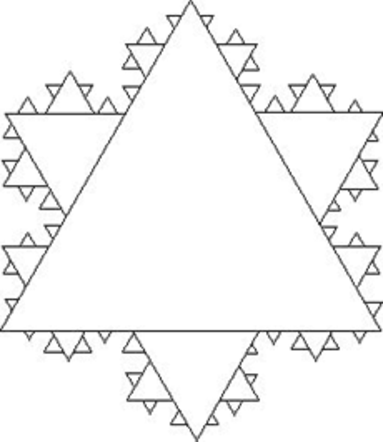
\includegraphics[width=0.2\textwidth]{figures/snowflake-triangle.pdf}
\end{center}
\caption{Koch snowflake drawn with triangles.}
\label{fig:snowflake-triangle}
\end{figure}

\begin{problemparts}
  \problempart \points{1} What is the depth of the recursion tree for rendering a
  snowflake of LoD $n$?
    \begin{enumerate}
      \item $\log n$
      \item $n$
      \item $3 \, n$
      \item $4 \, n$
    \end{enumerate}
\answerIa

  \problempart \points{2} How many nodes are there in the recursion tree at level
  $i$, for $1 \le i \le n$?
    \begin{enumerate}
     \item $3 ^ i$
      \item $4 ^ i$
      \item $4 ^ {i + 1}$
      \item $3 \cdot 4 ^ i$
    \end{enumerate}
\answerIb
    
  \problempart \points{1} What is the asymptotic rendering time (triangle count) for a
  node in the recursion tree at level $i$, for $0 \le i < n$?
    \begin{enumerate}
      \item $0$
      \item $\Theta(1)$
      \item $\Theta(\frac{1}{9}^i)$
      \item $\Theta(\frac{1}{3}^i)$
    \end{enumerate}
\answerIc 

  \problempart \points{1} What is the asymptotic rendering time (triangle count) at
  each level $i$ of the recursion tree, for $0 \le i < n$?
    \begin{enumerate}
      \item 0
      \item $\Theta(\frac{4}{9} ^ i)$
      \item $\Theta(3 ^ i)$
      \item $\Theta(4 ^ i)$
    \end{enumerate}
\answerId

  \problempart \points{2} What is the total asymptotic cost for the CPU, when rendering
  a snowflake with LoD $n$ using 3D hardware-accelerated rendering?
    \begin{enumerate}
      \item $\Theta(1)$
      \item $\Theta(n)$
      \item $\Theta(\frac{4}{3}^n)$
      \item $\Theta(4^n)$
    \end{enumerate}
\answerIe
\end{problemparts}

%\problempart
Second, when using 2D hardware-accelerated rendering, the surfaces'
outlines are broken down into open or closed paths (list of connected
line segments). For example, our snowflake is one closed path composed of
straight lines. The CPU compiles the list of cooordinates in each path to be
drawn, and sends it to the GPU, which renders the final image. This approach is
also used for talking to high-end toys such as laser cutters and plotters.

\begin{problemparts}
  \problempart \points{1} What is the depth of the recursion tree for rendering a
  snowflake of LoD $n$ using 2D hardware-accelerated rendering?
    \begin{enumerate}
      \item $\log n$
      \item $n$
      \item $3 \, n$
      \item $4 \, n$
    \end{enumerate}
\answerIf

  \problempart \points{1} How many nodes are there in the recursion tree at level
  $i$, for $1 \le i \le n$?
    \begin{enumerate}
      \item $3 ^ i$
      \item $4 ^ i$
      \item $4 ^ {i + 1}$
      \item $3 \cdot 4 ^ i$
    \end{enumerate}
\answerIg

  \problempart \points{1} What is the asymptotic rendering time (line segment count)
  for a node in the recursion tree at level $i$, for $0 \le i < n$?
    \begin{enumerate}
      \item $0$
      \item $\Theta(1)$
      \item $\Theta(\frac{1}{9}^i)$
      \item $\Theta(\frac{1}{3}^i)$
    \end{enumerate}
\answerIh

  \problempart \points{1} What is the asymptotic rendering time (line segment count)
  for a node in the last level $n$ of the recursion tree?
    \begin{enumerate}
      \item $0$
      \item $\Theta(1)$
      \item $\Theta(\frac{1}{9}^n)$
      \item $\Theta(\frac{1}{3}^n)$
    \end{enumerate}
\answerIi

  \problempart \points{1} What is the asymptotic rendering time (line segment count) at
  each level $i$ of the recursion tree, for $0 \le i < n$?
    \begin{enumerate}
      \item 0
      \item $\Theta(\frac{4}{9} ^ i)$
      \item $\Theta(3 ^ i)$
      \item $\Theta(4 ^ i)$
    \end{enumerate}
\answerIj

  \problempart \points{1} What is the asymptotic rendering time (line segment count) at
  the last level $n$ in the recursion tree?
    \begin{enumerate}
      \item $\Theta(1)$
      \item $\Theta(n)$
      \item $\Theta(\frac{4}{3}^n)$
      \item $\Theta(4^n)$
    \end{enumerate}
\answerIk

  \problempart \points{1} What is the total asymptotic cost for the CPU, when rendering
  a snowflake with LoD $n$ using 2D hardware-accelerated rendering?
    \begin{enumerate}
      \item $\Theta(1)$
      \item $\Theta(n)$
      \item $\Theta(\frac{4}{3}^n)$
      \item $\Theta(4^n)$
    \end{enumerate}
\answerIl

\end{problemparts}

%\problempart
Third, in 2D rendering without a hardware accelerator (also called
software rendering), the CPU compiles a list of line segments for each path like
in the previous part, but then it is also responsible for ``rasterizing'' each
line segment. Rasterizing takes the coordinates of the segment's endpoints and
computes the coordinates of all the pixels that lie on the line segment.
Changing the colors of these pixels effectively draws the line segment on the
display. We know an algorithm to rasterize a line segment in time proportional
to the length of the segment. It is easy to see that this algorithm is optimal,
because the number of pixels on the segment is proportional to the segment's
length. Throughout this problem, assume that all line segments have length
at least one pixel, so that the cost of rasterizing is greater than the cost
of compiling the line segments.

It might be interesting to note that the cost of 2D software rendering is
proportional to the total length of the path, which is also the power required
to cut the path with a laser cutter, or the amount of ink needed to print the
path on paper.

\begin{problemparts}
  \problempart \points{1} What is the depth of the recursion tree for rendering a
  snowflake of LoD $n$?
    \begin{enumerate}
      \item $\log n$
      \item $n$
      \item $3 \, n$
      \item $4 \, n$
    \end{enumerate}
\answerIm

  \problempart \points{1} How many nodes are there in the recursion tree at level
  $i$, for $1 \le i \le n$?
    \begin{enumerate}
      \item $3 ^ i$
      \item $4 ^ i$
      \item $4 ^ {i + 1}$
      \item $3 \cdot 4 ^ i$
    \end{enumerate}
\answerIn

  \problempart \points{1} What is the asymptotic rendering time (line segment length)
  for a node in the recursion tree at level $i$, for $0 \le i < n$? Assume that
  the sides of the initial triangle have length 1.
    \begin{enumerate}
      \item $0$
      \item $\Theta(1)$
      \item $\Theta(\frac{1}{9}^i)$
      \item $\Theta(\frac{1}{3}^i)$
    \end{enumerate}
\answerIo

  \problempart \points{1} What is the asymptotic rendering time (line segment length)
  for a node in the last level $n$ of the recursion tree?
    \begin{enumerate}
      \item $0$
      \item $\Theta(1)$
      \item $\Theta(\frac{1}{9}^n)$
      \item $\Theta(\frac{1}{3}^n)$
    \end{enumerate}
\answerIp

  \problempart \points{1} What is the asymptotic rendering time (line segment length)
  at each level $i$ of the recursion tree, for $0 \le i < n$?
    \begin{enumerate}
      \item 0
      \item $\Theta(\frac{4}{9} ^ i)$
      \item $\Theta(3 ^ i)$
      \item $\Theta(4 ^ i)$
    \end{enumerate}
\answerIq

  \problempart \points{1} What is the asymptotic rendering time (line segment length)
  at the last level $n$ in the recursion tree?
    \begin{enumerate}
      \item $\Theta(1)$
      \item $\Theta(n)$
      \item $\Theta(\frac{4}{3}^n)$
      \item $\Theta(4^n)$
    \end{enumerate}
\answerIr

  \problempart \points{1} What is the total asymptotic cost for the CPU, when rendering
  a snowflake with LoD $n$ using 2D software (not hardware-accelerated)
  rendering?
   \begin{enumerate}
      \item $\Theta(1)$
      \item $\Theta(n)$
      \item $\Theta(\frac{4}{3}^n)$
      \item $\Theta(4^n)$
    \end{enumerate}
\answerIs

\end{problemparts}

%\problempart
The fourth and last case we consider is 3D rendering without hardware
acceleration. In this case, the CPU compiles a list of triangles, and then
rasterizes each triangle. We know an algorithm to rasterize a triangle that
runs in time proportional to the triangle's surface area. This algorithm is
optimal, because the number of pixels inside a triangle is proportional to the
triangle's area. For the purpose of this problem, you can assume that the area
of a triangle with side length $l$ is $\Theta(l^2)$. We also assume that the
cost of rasterizing is greater than the cost of compiling the line segments.

\begin{problemparts}
  \problempart \points{4} What is the total asymptotic cost of rendering a snowflake
  with LoD $n$? Assume that initial triangle's side length is 1.
    \begin{enumerate}
      \item $\Theta(1)$
      \item $\Theta(n)$
      \item $\Theta(\frac{4}{3}^n)$
      \item $\Theta(4^n)$
    \end{enumerate}
\answerIt
    
  \problempart \points{15} Write a succinct proof for your answer using the  
  recursion-tree method.
  \answerIu
\end{problemparts}

%\end{problemparts}


\problem \points{60} \textbf{Digital Circuit Simulation}

Your 6.006 skills landed you a nice internship at the chip manufacturer AMDtel.
Their hardware verification team has been complaining that their circuit
simulator is slow, and your manager decided that your algorithmic chops make
you the perfect candidate for optimizing the simulator.

A \defn{combinational circuit} is made up of \defn{gates}, which are devices that take Boolean
($\mathsf{True}$ / 1 and $\mathsf{False}$ / 0) input signals, and output a
signal that is a function of the input signals. Gates take some time to compute
their functions, so a gate's output at time $\tau$ reflects the gate's inputs at
time $\tau - \delta$, where $\delta$ is the gate's delay. For the purposes of
this simulator, a gate's output transitions between 0 and 1 instantly. Gates'
output terminals are connected to other gates' inputs terminals by \defn{wires}
that propagate the signal instantly without altering it.

For example, a 2-input $\mathsf{XOR}$ gate with inputs A and B (Figure
\ref{fig:xor}) with a 2 nanosecond (ns) delay works as follows: 

\begin{center}
\begin{tabular}{|c|c|c|c|l|}
\hline
Time (ns) & Input A & Input B & Output O & Explanation \\
\hline
0 & 0 & 0 &   & Reflects inputs at time -2 \\ 
1 & 0 & 1 &   & Reflects inputs at time -1 \\ 
2 & 1 & 0 & 0 & 0 $\mathsf{XOR}$ 0, given at time 0 \\
3 & 1 & 1 & 1 & 0 $\mathsf{XOR}$ 1, given at time 1 \\
4 &   &   & 1 & 1 $\mathsf{XOR}$ 0, given at time 2 \\
5 &   &   & 0 & 1 $\mathsf{XOR}$ 1, given at time 3 \\
\hline
\end{tabular}
\end{center}

\begin{figure}[htbp]
\centering
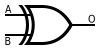
\includegraphics{figures/xor-ansi}
\caption{2-input $\mathsf{XOR}$ gate; $\mathsf{A}$ and $\mathsf{B}$ supply the
inputs, and $\mathsf{O}$ receives the output.}
\label{fig:xor}
\end{figure}  

The circuit simulator takes an input file that describes a circuit layout,
including gates' delays, probes (indicating the gates that we want to
monitor the output), and external inputs. It then simulates the transitions at
the output terminals of all the gates as time progresses. It also outputs
transitions at the probed gates in the order of the timing of those
transitions.

This problem will walk you through the best known approach for fixing
performance issues in a system. You will profile the code, find the performance
bottleneck, understand the reason behind it, and remove the bottleneck by
optimizing the code.

To start working with AMDtel's circuit simulation source code, download and
unpack the problem set's \texttt{.zip} archive, and go to the \texttt{circuit/}
directory.

The circuit simulator is in \texttt{circuit.py}. The AMDtel engineers pointed
out that the simulation input in \texttt{tests/5devadas13.in} takes too long
to run. We have also provided an automated test suite at
\texttt{test-circuit.py}, together with other simulation inputs. You can ignore
these files until you get to the last part of the problem set.

\begin{problemparts}

\problempart \points{8} Run the code under the python profiler with the command
below, and identify the method that takes up most of the CPU time. If two
methods have similar CPU usage times, ignore the simpler one.

\texttt{python -m cProfile -s time circuit.py < tests/5devadas13.in}

\textit{Warning:} the command above can take 15-30 minutes to complete, and
bring the CPU usage to 100\% on one of your cores. Plan accordingly.

What is the name of the method with the highest CPU usage?
\answerIIa

% CLI from http://docs.python.org/library/profile.html
% Sorting keys at http://docs.python.org/library/profile.html#profile-stats

\problempart \points{6} How many times is the method called?
\answerIIb

\problempart \points{8} The class containing the troublesome method is
implementing a familiar data structure. What is the tightest asymptotic bound
for the worst-case running time of the method that contains the bottleneck?
Express your answer in terms of $n$, the number of elements in the data
structure.
\begin{enumerate}
  \item $O(1)$.
  \item $O(\log n)$.
  \item $O(n)$.
  \item $O(n \log n)$.
  \item $O(n \log^2 n)$.
  \item $O(n^2)$.
\end{enumerate}
\answerIIc 

\problempart \points{8} If the data structure were implemented using the most
efficient method we learned in class, what would be the tightest asymptotic
bound for the worst-case running time of the method discussed in the questions
above?
\begin{enumerate}
  \item $O(1)$.
  \item $O(\log n)$.
  \item $O(n)$.
  \item $O(n \log n)$.
  \item $O(n \log^2 n)$.
  \item $O(n^2)$.
\end{enumerate}
\answerIId

\problempart \points{30} Rewrite the data structure class using the most
efficient method we learned in class. \textbf{Please note that you are not
allowed to import any additional Python libraries and our test will check this.}

We have provided a few tests to help you check your code's correctness and
speed. The test cases are in the \texttt{tests/} directory.
\texttt{tests/README.txt} explains the syntax of the simulator input files. You
can use the following command to run all the tests.

\texttt{python circuit\_test.py}

To work on a single test case, run the simulator on the test case with the
following command.

\texttt{python circuit.py < tests/1gate.in > out}

Then compare your output with the correct output for the test case.

\texttt{diff out tests/1gate.gold}

For Windows, use \texttt{fc} to compare files.

\texttt{fc out tests/1gate.gold}

We have implemented a visualizer for your output, to help you debug your code.
To use the visualizer, first produce a simulation trace.

\texttt{TRACE=jsonp python circuit.py < tests/1gate.in > circuit.jsonp}

On Windows, use the following command instead.

\texttt{circuit\_jsonp.bat < tests/1gate.in > circuit.jsonp}

Then use Google Chrome to open
\texttt{visualizer/bin/visualizer.html}

We recommend using the small test cases numbered 1 through 4 to check your
implementation's correctness, and then use test case 5 to check the code's
speed.

When your code passes all tests, and runs reasonably fast (the tests should
complete in less than 30 seconds on any reasonably recent computer), upload your
modified \texttt{circuit.py} to the course submission site.

\answer {
  Please upload \texttt{circuit.py} with your modifications separately.
}

\end{problemparts}

\end{problems}
\end{document}
